\chapter{Revisão Bibliográfica} \label{chap-levantamentoBibliografico}

O presente capítulo apresenta a revisão bibliográfica realizada,
apresentando na seção \ref{sec-jason} a plataforma Jason
em sua totalidade. Na seção \ref{sec-protocolo} são discutidos os
protocolos de serviços web considerados mais relevantes. Na seção
\ref{sec-relacionado} são apresentados trabalhos relacionados com o
que esta sendo proposto, discutindo suas diferenças com o presente.

\section{Jason} \label{sec-jason}

%Comentei esse todo, mas ele eh valido. Talvez desnecessario...
%\todo{de alguma forma, de2005planning deveriam estar
%contidos nesssa secao de revisao}
A plataforma Jason \cite{bordini-jason}, baseada na arquitetura BDI,
utiliza uma extensão da linguagem de programação abstrata \cite{rao1996agentspeak},
 chamada AgentSpeak(L), para especificar as decisões
dos agentes. Na seção \ref{sec-jason-overview} é apresentado uma
visão geral do Jason. Na seção \ref{sec-jason-architecture} é
debatido alguns detalhes da engenharia do Jason.

\subsection{Visão Geral} \label{sec-jason-overview}

Para explicar de forma mais didática será utilizado o
exemplo \emph{Room} que acompanha o Jason. Para isso será introduzido
o arquivo de projeto do exemplo e, a partir desse, os demais arquivos.
A Listagem~\ref{lst-roomMas2j} contém o arquivo de projeto.
Na linha 2, \emph{room} é o nome do projeto e, por isso, pode ser qualquer
identificador. A partir da linha 3 os valores antes dos dois-pontos (:)
são palavras reservadas que o Jason entende para diferentes propósitos e o valor
a seguir (depois dos dois-pontos) é o valor associado.
Assim, \emph{infrastructure}, na linha 3, pode assumir três valores
possíveis: (i) \emph{Centralised}, normalmente utilizada;
(ii) \emph{jade}, utilizada quando se deseja integrar
com agentes não Jason (jade); (iii) \emph{saci}, utilizada
quando deseja executar os agentes de maneira distribuída na rede.

%\lstset{linewidth=140mm}
\begin{center}
    \begin{minipage}{120mm}
	\begin{lstlisting}[frame=trbl, caption=Arquivo de projeto do Jason para o exemplo \emph{Room}, label=lst-roomMas2j]
// Isso eh um comentario
MAS room {
  infrastructure: Centralised
  environment: RoomEnv
  executionControl: jason.control.ExecutionControl
  agents: porter; claustrophobe; paranoid;
}
	\end{lstlisting}
    \end{minipage}
\end{center}

Continuando na Listagem~\ref{lst-roomMas2j}, a entrada \emph{environment}
configura a classe de ambiente que será utilizada. A próxima entrada,
normalmente não aparece, é a \emph{executionControl} utilizada para
mudar a forma com que os agentes são executados. O valor no exemplo é uma
classe que obriga o próximo ciclo de deliberação somente acontecer quando
todos os agentes terminaram o seu ciclo. O valor padrão é iniciar um novo
ciclo de deliberação após 500ms do ciclo de deliberação anterior ter sido
concluído, porém, algumas vezes isso
pode vir a apresentar problemas de sincronismo e, por isso, é interessante
mostrar que há uma opção para controlar a forma de execução dos ciclos
deliberativos. O usuário, inclusive, pode colocar sua própria classe como
configuração.

Todas as entradas apresentadas até agora mapeiam para código Java.
Os agentes são especificados na entrada \emph{agents}. Como pode-se
observar na Listagem~\ref{lst-roomMas2j}, cada referência a um agente deve
terminar com um ponto-e-vírgula (;). Há ainda como especializar cada um dos
agentes mudando opções. No capítulo \ref{chap-casoWS} será mostrado um exemplo
dessas opções.

Antes de entrar em discussão sobre os agentes será explicado o exemplo sendo
utilizado. No exemplo tem-se uma porta na sala e duas pessoas, uma
claustrofóbica e outra paranoica. A pessoa claustrofóbica deseja que a
porta da sala esteja aberta, enquanto que a paranoica deseja que a porta
fique fechada. Assim, os agentes Jason são desenvolvidos em arquivos texto
com extensão \emph{ASL} visando montar esse modelo.

Logo, há três agentes na linha 6 da Listagem~\ref{lst-roomMas2j}:
(i) \emph{porter} é o agente responsável pela porta e o único que conhece
como abri-lá ou fecha-lá;
(ii) \emph{claustrophobe} é o agente que deseja deixar a porta sempre aberta;
(iii) \emph{paranoid} é o agente que deseja deixar a porta sempre fechada.
A implementação desses agentes torna-se muito simples com o uso de eventos.

Esses eventos podem ser de adição (+) ou de remoção (-) de crenças, metas ou
consultas. Todas as estruturas são semelhantes a chamada de função. No
exemplo ``telefone(808080822)'', telefone pode ser uma crença ou uma ação de
ambiente que pode ser executada dependendo de onde a entrada se localiza.
Note que, se essa entrada for precedida pelo sinal de exclamação (!) ou de
interrogação (?) então o significado é alterado respectivamente para uma meta
ou uma consulta. Ainda há a possibilidade de preceder uma crença ou meta
com sinal de adição ou de subtração significando ou adicionar/remover uma
crença ou estar recebendo/removendo uma crença, meta ou consulta.

\lstset{linewidth=75mm}
\begin{wrapfigure}{l}{85mm}
	\begin{lstlisting}[frame=trbl, caption=Agentes em ASL, label=lst-agente]
// claustrophobe.asl
+locked(door) : true
  <- .send(porter,achieve,~locked(door)).

// paranoid.asl
+~locked(door)
  <- .send(porter,achieve,locked(door)).

// porter.asl
+!locked(door)[source(paranoid)]
  : ~locked(door)
  <- lock.

+!~locked(door)[source(claustrophobe)]
  : locked(door)
  <- unlock.
	\end{lstlisting}
\end{wrapfigure}
%
Na Listagem~\ref{lst-agente} tem-se a continuação do exemplo e, por
simplicidade, todos os fontes dos agentes encontram-se reunidos. O agente denominado
\emph{claustrophobe} será o primeiro a ser detalhado e corresponde as linhas 1 até 3
da Listagem~\ref{lst-agente}. A programação em Jason é
guiada por reatividade nas crenças e percepções do próprio agente, assim, é necessário
uma forma de estruturar as ações à serem decididas. Essa forma é o plano.
O plano pode ser ativado quando se deseja adicionar, consultar ou remover \footnote{Uma remoção pode ser o momento de conter uma falhar, porém isso não será abordado.}
 uma crença ou meta. O plano da linha 2 até 3 da
Listagem~\ref{lst-agente} será detalhado adiante.

Em um plano há sempre três divisões: gatilho do evento, contexto e corpo.
A primeira e única à ser explicita é o gatilho do evento, que deve ocorrer para
o plano ser disparado. No exemplo ele está limitado do carácter inicial até
o dois-pontos (:). A divisão de contexto é onde se coloca as ações, crenças
ou regras de inferência que tem que ser válidas para o corpo do plano ser
considerado válido. Dessa forma, é
importante tomar cuidado no que vai no contexto em razão dele sempre ser
executado previamente para definir quais planos devem ser descartados.
A segunda divisão vai até a seta (<-) e não é obrigatória.
A terceira divisão, também não é obrigatória, possui todas as ações a serem executadas pelo
seu plano. No exemplo o plano tem em seu corpo uma ação interna do Jason
denominada \emph{send} que envia determinado dado (terceiro parâmetro) para o
agente especificado (primeiro parâmetro) com determinado formato (segundo parâmetro).

Cabe chamar atenção para uma coisa, as ações internas podem ser definidas pelo
usuário. Uma ação interna possui o seguinte formato ``tcp.send'', assim essa
ação está definida no pacote \emph{tcp} pela classe \emph{send} que
deve especializar a classe \emph{DefaultInternalAction} do Jason.
Entretanto, uma ação interna definida pelo Jason não possui indicativo de
pacote que é o caso do ``.send'' presente no código dos agentes.

No exemplo da linha 3 na Listagem~\ref{lst-agente}, o agente
\emph{claustrophobe} está enviando uma mensagem para o agente denominado \emph{porter}
ter a meta (\emph{achieve} no segundo parâmetro) de não ($\sim$) ter a crença
da porta estar fechada. Analogamente, o agente denominado \emph{paranoid}, definido
na linha 5 à 7, envia como crença ter a porta fechada. Logo, o agente \emph{porter} pode ser entendido
em sua quase totalidade na Listagem~\ref{lst-agente}. Um entendimento completo
do exemplo vem com o aprendizado das anotações que são dados que podem
ser guardados juntos das crenças e essas anotações podem ter suas anotações também.
No agente \emph{porter} essas anotações são utilizadas somente
para dizer que determinado plano só é válido quando tiver como fonte 
(do inglês \emph{source}) um determinado agente. O presente exemplo possui
as anotações, pois assume a hipótese do mundo aberto. Vale observar que, essas
anotações podem ser removidas sem nenhum problema adicional, visto que, no
mundo proposto o agente \emph{porter} recebe a meta a ser alcançada de um dos
dois agentes existentes.

A execução dos agentes acontece de forma arbitrária e deve-se ter em conta
que o primeiro agente que irá enviar a mensagem para o agente \emph{porter} dependerá
de como o mundo inicia. Logo, se o mundo iniciar com a porta fechada o primeiro
a enviar a solicitação será o agente \emph{claustrophobe}. Já se o mundo for iniciado
com a porta aberta o primeiro a enviar solicitação será o agente \emph{paranoid}.
Além disso, conforme a simulação vai correndo os dois agentes ficam alternando
mensagens com o agente \emph{porter} por causa do compartilhamento do mesmo recurso.

\subsection{Infra-estrutura do Jason} \label{sec-jason-architecture}

A plataforma Jason tem uma base de software completamente extensível como
é possível observar mediante a Figura \ref{fig-jason-infra-1}.
Nessa figura, a infra-estrutura encontra-se representada como um barramento
na parte inferior. Ela pode ser configurada através da chave de configuração
\emph{infrastructure} no arquivo de projeto (ver Listagem~\ref{lst-roomMas2j}).

A infraestrutura define todas as classes padrões que o usuário irá utilizar,
por exemplo observe que o barramento liga-se a dois adaptadores: um do tipo
agente e um de ambiente. Esses adaptadores permitem a compatibilidade entre
implementações distintas de classes permitindo que as implementações não
padrão variem sem ter que alterar a estrutura do barramento.

\begin{figure}
               \begin{center}
               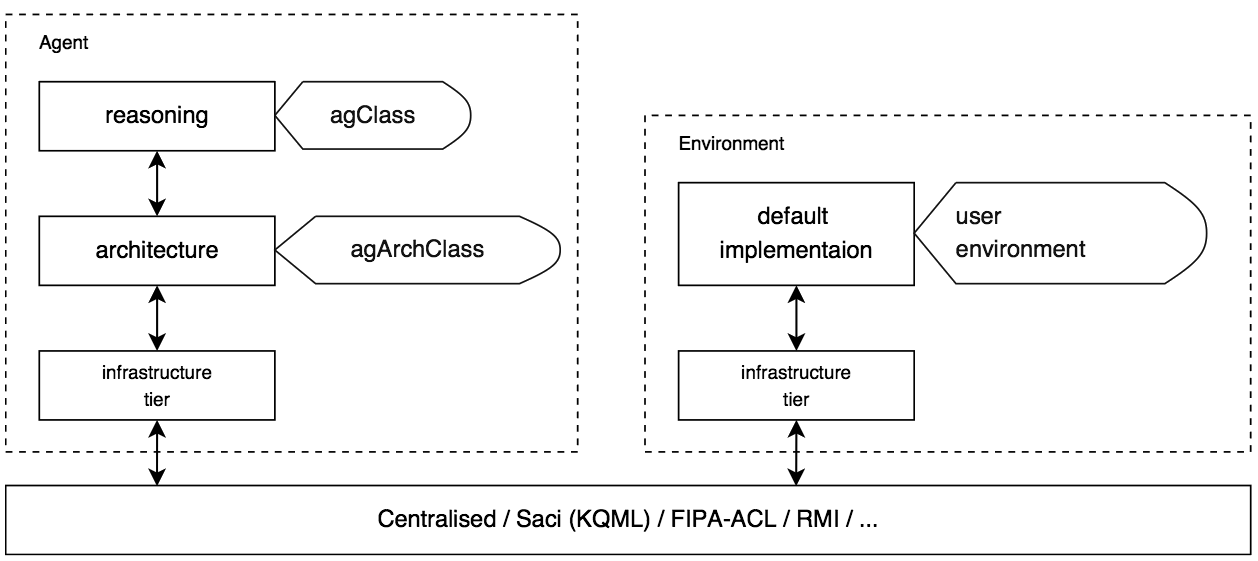
\includegraphics[width=140mm]{figuras/infra.png} 
                \end{center}
                \caption{Modelo da infra-estrutura do Jason.}
                \label{fig-jason-infra-1}
\end{figure}

Assim, há a possibilidade de informar para uma determinada simulação que um
determinado agente utilizará uma arquitetura e/ou um raciocinador diferente
dos demais agentes. Para se fazer isso no momento que se declara os agentes
no projeto informa-se as chaves que encontram-se dentro das caixas com
cantos arqueados na Figura~\ref{fig-jason-infra-1}. O exemplo
``fb agArchClass KosMos.FireBrigadeArch agClass KosMos.Agent \#1;'' define
o agente \emph{fb} com a arquitetura usando a classe \emph{FireBrigadeArch}
do pacote \emph{KosMos} (pode ser qualquer nome desejado) e utilizando como
raciocinador a classe \emph{Agent} do mesmo pacote. Note que, essas classes
não existem no Jason e devem ser providas pelo usuário de alguma forma.

Como já explicado, a entrada \emph{environment} no arquivo de projeto
configura a classe de ambiente que será utilizada. Assim, somente um ambiente
é permitido por simulação. Um dos motivos comuns de se implementar um
ambiente é implementar as ações que o agente poderá realizar. Porém,
também é possível alterar como os agentes ``visualizam'' o ambiente. Um
agente pode ser implementado deixando as ações tanto em uma
especialização da infraestrutura quanto direto no ambiente. Por ser o
ambiente, o responsável pelas percepções então seria nele que a implementação
de falhas em sensores ocorreria. Essas falhas podem ser implementadas através
da remoção ou alteração das percepções. O agente, nesse ambiente, deveria ser
capaz de aplicar regras para verificar essas falhas e assumir que há erros em
seus dados.

\section{Protocolos de serviços web} \label{sec-protocolo}

Os protocolos de serviços web são todos baseados no conceito pergunta-resposta.
Esse conceito é a base da internet hoje através de inúmeros protocolos de
transferência de dados. Dentre esses protocolos, o de maior destaque para o
presente trabalho é o protocolo HTTP (\emph{Hyper} \emph{Text} \emph{Transfer}
\emph{Protocol}) \footnote{Veja a RFC-1945 e RFC-2616 para maiores detalhes.}.

A comunicação do protocolo HTTP considera que sempre há duas entidades: o
solicitante e o atendente. O solicitante envia algum dos comandos possíveis
ao atendente que é responsável por interpretar o comando enviado e responde-lo
adequadamente. Essa comunicação é ilustrada na Figura~\ref{fig-http} que mostra
uma solicitação de uma página da web através de um dos comandos possíveis
no protocolo HTTP.

\begin{figure}
	\begin{center}
	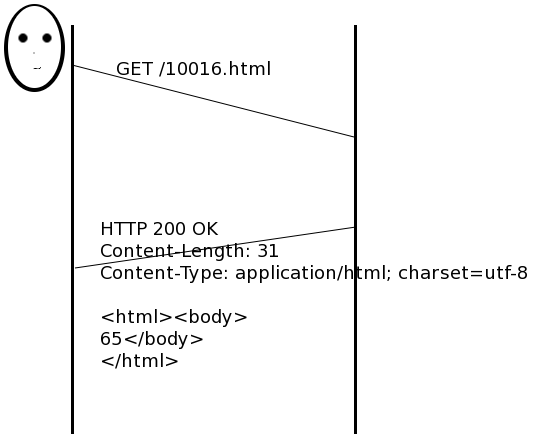
\includegraphics[width=60mm]{figuras/http-request.png} 
	\end{center}
	\caption{Exemplo de requisição HTTP, o ator (o solicitante) na esquerda e a direita o servidor que responde (o atendente).}
	\label{fig-http}
\end{figure}

A troca de informações, no protocolo HTTP, é realizada sempre via texto puro.
Assim, a presente seção explica os protocolos de serviços web que são
os mais conhecidos baseados na linguagem XML \footnote{Abordar a linguagem
XML esta fora de escopo, visite http://www.w3.org/TR/xml/ para mais detalhes.}
que podem ser utilizados sobre esse protocolo.
Na subseção \ref{sec-protocolo-xmlrpc} introduz-se o protocolo XML-RPC e na
subseção \ref{sec-protocolo-soap} debate-se o SOAP.

\subsection{XML-RPC} \label{sec-protocolo-xmlrpc}

O XML-RPC surgiu em meados de 1998 visando permitir que funções ou procedimentos
fossem feitos através de rede sobre o protocolo HTTP \cite{cerami2002web}. Dessa
forma, um programa cliente
pode passar informações à um dado servidor com uma pequena descrição de sua
solicitação e o servidor responde com uma falta ou com uma mensagem descrevendo
o retorno propriamente dito. Uma falta é equivalente a um erro ou exceção podendo
ter caráter temporário (base de dados sobrecarregada) ou permanente (requisição
sendo feita é inválida).

O protocolo XML-RPC define 8 tipos de dados que podem ser utilizados
tanto nos valores de parâmetros, quanto de retornos ou de faltas. Esses
tipos encontram-se representados na Tabela~\ref{table-xmlrpc-data}. Dentre
esses tipos de dados, os mais complexos são ``<struct>'' e ``<array>''. Nestes,
ambos, admitem em sua valoração qualquer dos tipos de dados possíveis (inclusive
seu próprio). Sobre o ``<array>'' não há uma obrigação de utilizar em
sua valoração o mesmo tipo em todos os seus elementos. Toda a informação trocada
é textual e deve estar claro que é responsabilidade do solicitante e/ou do servidor saber
traduzir da sua forma de armazenamento para texto ou vice-versa.

\lstset{linewidth=75mm}
\begin{wrapfigure}{l}{85mm}
    \begin{minipage}{75mm}
	\begin{lstlisting}[frame=trbl, caption=Exemplo de chamada XML-RPC com os cabeçalhos HTTP sendo omitidos \cite{cerami2002web}., label=lst-xmlrpc-req]
<?xml version="1.0" encoding="UTF-8" ?>
<methodCall>
 <methodName>getWeather</methodName>
 <params>
  <param>
   <value><string>10016</string></value>
  </param>
 </params>
</methodCall>
	\end{lstlisting}
	\end{minipage}
\end{wrapfigure}

As descrições que podem ser utilizadas tanto pelo solicitante quanto pelo servidor
são fundamentais. O protocolo descreve duas estruturas primordiais relativas aos
métodos. A primeira delas é a chamada de métodos que inicia com ``<methodCall>''
devendo conter um ``<methodName>'' que conterá o nome do procedimento sendo
realizado. Quando o procedimento contiver parâmetros, eles devem estar contidos em
``<params>'' e para cada parâmetro um ``<param>'' contendo ``<value>'' deve
ser informado. O valor do parâmetro pode ser qualquer um dos 8 tipos
de dados possíveis (ver Tabela~\ref{table-xmlrpc-data}).
Um exemplo dessa estruturação pode ser vista na Listagem~\ref{lst-xmlrpc-req}.

\begin{table}
	\caption{Tipos de dados no XML-RPC.}
	\label{table-xmlrpc-data}
	\begin{center}
	\begin{tabular}{|p{34mm}|p{50mm}|p{50mm}|}
		\hline
		Etiqueta & Descrição & Exemplo \\ \hline
		<i4> ou <int> & Inteiro sinalizado de 4 bytes. & \scriptsize{<i4>-21</i4>} \\ \hline
		<boolean> & 0 (falso) ou 1 (verdadeiro). & \scriptsize{<boolean>1</boolean>} \\ \hline
		<string> & Texto. & \scriptsize{<string>Ricardo Lucca</string>} \\ \hline
		<double> & Valor de ponto flutuante com precisão dupla. & \scriptsize{<double>-21.145</double>} \\ \hline
		<dateTime.iso8601> & Data e Tempo. & \scriptsize{<dateTime.iso8601>\newline\hspace*{1mm}20100924T12:26:35\newline</dateTime.iso8601>} \\ \hline
		<base64> & Texto codificado em base 64. & \scriptsize{<base64>\newline\hspace*{1mm}bWUgYXByb3ZhcmVpPw==\newline</base64>} \\ \hline
		<struct> & Estrutura com membros e cada membro com nome e um valor associado. & \scriptsize{<struct>\newline\hspace*{1mm}<member>\newline\hspace*{2mm}<name>weather</name>\newline\hspace*{2mm}<value><int>65</int></value>\newline\hspace*{1mm}</member>\newline\hspace*{1mm}...\newline</struct>} \\ \hline
		<array> & Vetor com valores. & \scriptsize{<array><data>\newline\hspace*{1mm}<value><boolean>0</boolean></value>\newline\hspace*{1mm}<value><int>65</int></value>\newline\hspace*{1mm}...\newline</data></array>} \\ \hline
	\end{tabular}
	\end{center}
\end{table}

Já, a segunda estrutura primordial é a de resposta do método e é iniciada
com ``<methodResponse>''. Os valores retornados pelo método são análogos aos
parâmetros de chamada, isto é, devem estar em ``<params>'' e para cada valor
retornado um ``<param>'' contendo ``<value>'' deve existir com um tipo de dado.
Um exemplo de resposta pode ser visto na Listagem~\ref{lst-xmlrpc-resp}.

Um método, também pode retornar uma falta.
Para isso o elemento raiz deve ser ``<methodResponse>'' por ser uma resposta
de método e ao invés de ``<params>'' no interior será utilizado o elemento
``<fault>''. Assim, normalmente, quando a implementação deseja devolver
detalhes do erro, uma estrutura ou vetor para conter maiores detalhes sobre o
mesmo pode ser utilizada.

\lstset{linewidth=85mm}
\begin{wrapfigure}{l}{95mm}
    \begin{minipage}{85mm}
	\begin{lstlisting}[frame=trbl, caption=Exemplo de resposta XML-RPC com os cabeçalhos HTTP sendo omitidos \cite{cerami2002web}., label=lst-xmlrpc-resp]
<?xml version="1.0" encoding="UTF-8" ?>
<methodResponse>
 <params>
  <param>
   <value><int>65</int></value>
  </param>
 </params>
</methodResponse>
	\end{lstlisting}
	\end{minipage}
\end{wrapfigure}

Em \cite{allman2003evaluation}, uma analise do uso do XML-RPC tanto do
ponto de tráfego de rede quanto de complexidade de código foi realizada.
O estudo mostrou que para um pequeno volume de dados a ser transmitido e
recebido, onde há pouca interação entre os participantes, o uso do XML-RPC
seria equivalente à utilização de comunicação via \emph{sockets}. Entretanto,
em cenários onde o volume de dado é maior se torna bastante desparelho a
utilização de XML-RPC contra \emph{sockets}. Os dados comunicados via
\emph{sockets} podem ser em formato binário com a menor redundância possível,
porém ao utilizar XML-RPC uma representação textual do dado é necessária e,
sempre, mesmo que pequeno, haverá redundância na informação de marcação.
%\todo{me veio na cabeca, aqui eu nao deveria falar tb um pouco sobre o desenvolvimento?}

\subsection{SOAP} \label{sec-protocolo-soap}

O SOAP                                 é o nome de um protocolo análogo ao XML-RPC.
Ele surgiu em março do ano 2000, porém não descreve em nenhum momento como objetos
devem estar definidos para serem reconstruídos nas entidades
envolvidas \cite{cerami2002web}. O nome SOAP foi mantido pela W3C por se tratar
de um protocolo que se destacou rapidamente por sua forte ligação com o XML Schema.

O protocolo SOAP descreve a comunicação entre cliente e servidor como sendo uma serie
de mensagens SOAP. Essas mensagens são, basicamente, envelopes com o conteúdo a ser
enviado. Cada envelope deve conter um corpo que é onde fica as informações do que
deve ser feito e podem conter uma seção com informações adicionais para a aplicação.
Além disso, a seção do corpo pode conter uma seção de falta, semelhante a
forma do XML-RPC.

Antes de apresentar exemplos das mensagens SOAP, trocadas entre o cliente e o
servidor, cada uma das seções da mensagem será abordada.
A primeira seção chamada de envelope
é o elemento raiz das mensagens SOAP. Essa seção é iniciada com
``<SOAP-ENV:Envelope>'' e nela contêm um controle de versão através do uso de
\emph{namespace} utilizando o atributo ``xmlns:SOAP-ENV'' \footnote{Note que no XML-RPC não existe essa preocupação}. Caso o
\emph{namespace} informado não seja válido a mensagem pode ser ignorada.

A seção seguinte é chamada \emph{Header} e pode conter informações adicionais úteis
para a aplicação. Essa seção não esta presente na maioria das mensagens e,
dessa forma,
ao prover uma determinada informação é possível indicar que o
o não entendimento desta ocasione a falha do método. Assim, isso pode
servir para diferentes propósitos. O elemento ``<SOAP-ENV:Header>''
define a raiz desta seção.

O corpo da mensagem é definido por ``<SOAP-ENV:Body>'' e
será explicado juntamente com os exemplos. Lembra-se ainda que,
dentro da seção corpo há uma em especial que trata
de falha e é definido pelo ``<SOAP-ENV:Fault>''. Esse elemento pode conter 4 elementos que
descrevem o erro: \emph{faultcode}, o tipo de erro acontecido; \emph{faultstring}, a
descrição do erro acontecido; \emph{faultactor}, onde aconteceu a falha \footnote{Uma mensagem SOAP pode ser reenviada para outro servidor conhecido sem informar o usuário disso. Esse roteamento está fora do escopo e está sendo mencionado a título de curiosidade.}; \emph{detail}, um campo livre
utilizado para enviar dados de volta para a aplicação. Quando acontece uma falta esse
é o único elemento que pode vir dentro do corpo da mensagem, os dados que descrevem o
erro podem variar. Por exemplo, ser retornado \emph{faultstring} e \emph{detail}
ou somente \emph{faultstring} ou outra combinação dos elementos explicados.

A Listagem~\ref{lst-soap-req} demostra uma chamada SOAP sendo feita. No envelope
da mensagem tem-se três \emph{namespaces} informados, um deles utilizado para
versionamento do SOAP (atributo ``xmlns:SOAP-ENV'') e outros dois utilizados
para descrever as versões da codificação dos dados em XML Schema (atributos
``xmlns:xsi'' e ``xmlns:xsd''). Além disso, dentro da seção de corpo da mensagem
ha mais um \emph{namespace} definido pelo atributo ``xmlns:ns1'' no método
sendo chamado, no exemplo \emph{getWeather} definido por ``<ns1:getWeather>''.
Esse último \emph{namespace} pode ser utilizado pela aplicação para fazer
uma diferenciação entre métodos com versões diferentes.

\lstset{linewidth=140mm}
\begin{center}
    \begin{minipage}{140mm}
	\begin{lstlisting}[frame=trbl, caption=Exemplo de chamada SOAP com os cabeçalhos HTTP sendo omitidos \cite{cerami2002web}., label=lst-soap-req]
<?xml version="1.0" encoding="UTF-8"?>
<SOAP-ENV:Envelope
 xmlns:SOAP-ENV="http://www.w3.org/2001/09/soap-envelope/"
 xmlns:xsi="http://www.w3.org/2001/XMLSChema-instance"
 xmlns:xsd="http://www.w3.org/2001/XMLSChema">
 <SOAP-ENV:Body>
  <ns1:getWeather xmlns:ns1="urn:examples:weatherservice"
   SOAP-ENV:encodingStyle="http://www.w3.org/2001/09/soap-encoding/">
    <zipcode xsi:type="xsd:string">10016</zipcode>
  </ns1:getWeather>
 </SOAP-ENV:Body>
</SOAP-ENV:Envelope>
	\end{lstlisting}
	\end{minipage}
\end{center}

Todas as mensagens SOAP tem um envelope como sendo a forma primordial. Dentro
desse, existe uma seção com dados adicionais e/ou uma seção com o corpo
da mensagem. No corpo da mensagem cada um dos seus sub-elementos são métodos
que estão sendo chamados e cada sub-elemento desses sub-elementos correspondem
aos parâmetros do método. Assim, na Listagem~\ref{lst-soap-req} há um único método sendo
chamado de nome \emph{getWeather} e um parâmetro de nome \emph{zipcode} do
tipo ``xsd:string'' definido pelo atributo ``xsi:type'' valendo 10016. Se houvessem
mais parâmetros desse métodos, eles viriam todos no mesmo nível do \emph{zipcode}.
No exemplo foi utilizado um dos tipos de codificação de parâmetros possíveis, porém
isso é configurado em cada um dos métodos através do atributo ``SOAP-ENV:encodingStyle''.

Todos os tipos de dados do XML Schema
podem ser utilizados. Assim, qualquer um dos 50 tipos possíveis podem
ser utilizados no envio de dados via SOAP. Entre esses há tipos complexos
como os vetores e estruturas que seriam equivalentes aos do XML-RPC,
mas com formas de utilização diferentes.

A descrição da resposta do método é análoga a descrição de chamada do
método, pois ambas são mensagens SOAP. Na resposta, tem-se um envelope
encapsulando informações tanto adicionais quanto do corpo da mensagem.
O corpo da mensagem tem como elemento raiz o elemento ``<SOAP-ENV:Body>'',
porém cada um dos sub-elementos serão respostas de métodos solicitados
e cada sub-elemento destes serão os valores de retorno do método.

Na Listagem~\ref{lst-soap-resp}, o elemento ``ns1:getWeatherResponse'' é a
resposta do método.
Ele possui apenas um valor retornado definido
como sendo um inteiro através do atributo``xsi:type'' com valor 65. O tipo
inteiro é um tipo simples, porém, quando retornado um tipo complexo como
sub-elemento de ``<return>'' pode haver necessidade do uso de etiquetas
correspondentes ao tipo em questão.
Por exemplo, no caso de vetores as etiquetas seriam
``<item>'' e, no caso de ser devolvido uma estrutura, cada etiqueta assumiria
o nome do membro sendo sendo retornado.

Em \cite{kohlhoff2003evaluating}, uma analise do SOAP foi realizada visando
performance no tráfego da rede. Durante o trabalho, o autor comenta
que é normal um aumento de até 10 vezes na representação textual
dos dados, quando comparado com o tamanho do dado em sua forma binária. Declara,
ainda, que, o principal ponto
onde o SOAP gasta tempo é nas conversões entre representação binária e
textual e vice-versa.
Entretanto, ele conclui que com um tamanho de pacote de comunicação maior, a
vantagem pode ser do SOAP.
Dessa forma, pacotes muito pequenos seriam atrasados e o SOAP
não sofreria atrasos.
%\todo{me veio na cabeca, aqui eu nao deveria falar tb um pouco sobre o desenvolvimento?}

\lstset{linewidth=120mm}
\begin{center}
    \begin{minipage}{120mm}
	\begin{lstlisting}[frame=trbl, caption=Exemplo de chamada SOAP com os cabeçalhos HTTP sendo omitidos \cite{cerami2002web}., label=lst-soap-resp]
<?xml version="1.0" encoding="UTF-8"?>
<SOAP-ENV:Envelope
 xmlns:SOAP-ENV="http://www.w3.org/2001/09/soap-envelope/"
 xmlns:xsi="http://www.w3.org/2001/XMLSChema-instance"
 xmlns:xsd="http://www.w3.org/2001/XMLSChema">
 <SOAP-ENV:Body>
  <ns1:getWeatherResponse xmlns:ns1="urn:examples:weatherservice"
   SOAP-ENV:encodingStyle="http://www.w3.org/2001/09/soap-encoding/">
   <return xsi:type="xsd:int">65</return>
  </ns1:getWeatherResponse>
 </SOAP-ENV:Body>
</SOAP-ENV:Envelope>
	\end{lstlisting}
	\end{minipage}
\end{center}

\section{Trabalhos relacionados} \label{sec-relacionado}

Trabalhos com agentes distribuídos existem os mais diversos
\cite{bellifemine1999jade,Buhler03adaptiveworkflow,piunti2009soa}. Entre
esses trabalhos, o Jade é um \emph{framework} que utiliza o protocolo FIPA.
Esse protocolo define formas de interação entre os diferentes agentes
\cite{bellifemine1999jade} e não como a interação ocorre. Observe, também,
que o tempo entre a interação entre agentes para realocar tarefas é um fator
crítico.

O Jade permite que agentes estejam dispersos utilizando a tecnologia
RMI \footnote{\emph{Remote Method Interface} é
um mecanismo análogo ao RPC, porém para orientação à objetos.}. A execução
de ações é através da adição e remoção de comportamentos. Esses
podem ser de dois tipos: (i) simples; (ii) complexos. O comportamento simples
equivale a uma ação executada sem interrupção que pode ser repetida até
se obter o que se deseja. O comportamento complexo é um comportamento que pode
ser interrompido e possui regras de pré e pós execução. Dessa forma, esse
comportamento pode ser uma cadeia de ações a serem executadas em sequência ou
de maneira não determinística. O Jason já possui uma forma de utilizar o Jade
em seu ambiente, porém o uso do RMI não atende aos critérios do presente
trabalho, visto que o RMI obrigaria a utilização de uma linguagem com
orientação a objetos, porém, um dos critérios do presente trabalho é a
independência de paradigma.

Em \cite{Buhler03adaptiveworkflow} o protocolo FIPA é utilizado na coordenação
de agentes. Os servidores de serviço Web (WSS) possuem os recursos
computacionais que são alocados
para determinadas tarefas e os agentes decidem que tarefas serão alocadas para
esses WSS. O conceito chave aqui é ``atividades + coordenação'' sendo que as
atividades são realizadas pelos WSS e a coordenação (social) pelos agentes. A
linguagem utilizada para descrever a coordenação foi uma linguagem de negócio.
Esse trabalho é fortemente relacionado com o nosso, mas o objetivo dele é
apenas coordenar os agentes em alto nível para se ter uma sociedade da melhor
forma possível. Nossa meta é permitir que a plataforma Jason seja aberta e
possa receber agentes e ambientes em diferentes linguagens seja ela orientada
ou não à negócios e/ou à objetos.

O Cartago tem a finalidade de ser um meio de campo entre o agente e o
ambiente \cite{ricci31cartago}. Assim, para descrever o ambiente, duas
abstrações de primeira classe são utilizadas. A primeira abstração é o agente
que é o ator (ou personagem) existente no ambiente. Ele tem a capacidade de
interagir ou criar os objetos com que vai trabalhar de maneira dinâmica. A
segunda abstração é chamada de artefato e refere-se aos objetos que estão no
mundo e podem ser utilizados pelo agente. Dessa forma, se um agente deseja
interagir com um determinado artefato existe uma interface padrão que permite
diversas formas de interação. Por exemplo, o agente pode ficar focado em um determinado
artefato para receber notificações de mudanças no mesmo ou pode
registrar interesse em propriedades especificas para quando houver modificação
ser notificado e, ainda, pode executar ações especificas proporcionadas pelo
artefato.

O Cartago-WS \cite{piunti2009soa} estende o Cartago com a finalidade de
permitir que os artefatos sejam WS. Dessa forma, uma ação solicitada
pelo agente pode ser exercida por um artefato que nem mesmo encontra-se na
mesma máquina. Há uma serie de extensões possíveis de serem utilizadas que
permitem características diferentes, por exemplo, coordenação e segurança.
O Cartago-WS foi feito utilizando JAX-WS
\footnote{\emph{Java Api for Xml Web Service}. Veja mais em
http://java.sun.com/developer/technicalArticles/J2SE/jax\_ws\_2/.} baseado na
tecnologia SOAP. Conforme mencionado no Capítulo \ref{chap-introducao}, o
presente trabalho se baseara diretamente na tecnologia SOAP ou na XML-RPC.
Além disso, tanto os objetos quanto os agentes na implementação sendo proposta
podem ser WS, enquanto, que no Cartago-WS somente os objetos.

